%%%%%%%%%%%%%%%%%%%%%%%%%%%%%%%%%%%%%%%%%%%%%%%%%%%%%%%%%%%%
\section{$WW$ and $WZ$ analysis}
This section describes the study of diboson production, $WW$ and $WZ$, in events with a leptonically 
decaying $W$ boson  ($W\to\ell\nu$, $\ell=e,\mu$) and one other 
$W$ or $Z$ boson that decays to $q\bar{q}$.

\par
The advantage of reconstructing $WW$ + $WZ$ in $\ell\nu jj$ decay mode over 
the purely leptonic channels is the larger branching fraction to jets, 
at the expense of larger backgrounds, mainly from $W$+jets.
Compared to the pure $WW$ leptonic diboson decay the semi-leptonic 
process has the ability to  provide a direct handle on the boson transverse 
momentum. 
The sensitivity to very high boson $p_T$ makes this process particularly 
useful as a probe of the gauge symmetries at high energies 
where we anticipate new physics.
On the flip side, this channel is beset by a large background from 
single $W$ boson produced in association with quarks and/or gluons.

\par
The sample is dominated by associated production of $W$ boson 
with two or more jets, but also contains diboson events with hadronic 
$W$ or $Z$ decay to two jets ($W/Z\to jj$), 
and small contribution from 
top pair ($\ttbar\to l\nu jj$), single top ($pp\to tq \to \ell\nu jj$),
and QCD multijet events. 
We analyze data sample corresponding to an integrated 
luminosity of 1 fb${}^{-1}$.
Electron or muon from the leptonic decay of the $W$ is used to trigger 
the event (along with requirement on $\met$ and hadronic activity).
The shape of dijet mass spectrum is used to discriminate the hadronic 
$W/Z\to jj$  decay from the $W$+jets, $\ttbar$, single top, and QCD multijet 
processes.


\subsection{Event selection\label{sec:evtSel}}
\subsubsection{Leptons \label{sec:leptonId}}
\par
Electrons are identified from a clusters of electromagnetic 
calorimeter (ECAL) energy deposits
matched to tracks from the silicon tracker. 
They must fall in the ECAL fiducial volume of $|\eta| < 2.5$ 
excluding the transition region $1.44 < |\eta| < 1.57$ 
between the barrel and endcap, and the trsnsverse energy $\et$ 
should be more than $30~\gev$.
Electron tracks are reconstructed using an
algorithm~\cite{GSF} that accounts for possible energy loss due to
bremsstrahlung in the tracker layers.
The energy of an electron candidate with $\et>30~\gev$ is essentially
determined by the ECAL cluster energy, while its momentum direction
is determined by that of the associated track.

\par
Particles misidentified as electrons are 
suppressed by requiring that the $\eta$ and $\phi$ coordinates
of the track trajectory extrapolated to the ECAL match the $\eta$ and
$\phi$ coordinates of the ECAL cluster, by requiring a narrow ECAL
cluster width in $\eta$, and by limiting the HCAL energy measured in a
cone of $\Delta R < 0.15$ around the ECAL cluster direction.
Electrons from photon conversions are suppressed by requiring
one hit in the innermost pixel layer for the
reconstructed electron track.  Furthermore, electrons are
rejected when a partner track is found that is consistent with a
photon conversion, based on the opening angle and the separation in
the transverse plane at the point at which the electron and partner
tracks are parallel. More details and studies of electron reconstruction
and identification can be found in Ref.~\cite{CMS-PAS-EGM-10-004}.


\par
Muons candidates are identified by two different 
algorithms~\cite{MUONPAS}: one proceeds from the inner tracker outwards, 
the other one starts from tracks measured in the muon chambers and matches 
and combines them with tracks reconstructed in the inner tracker. 
Muon candidates are requires to have $|\eta| < 2.4$.
Muons from decays in flight of hadrons and punch-through particles are 
reduced applying a cut of $\chi^2/ndof < 10$
on a global fit including tracker and muon detector hits.
In order to ensure a precise estimate of momentum and impact parameter
only tracks with more than 10 hits in the inner tracker and at least 
one hit in the pixel detector are used.
We require hits in at least two muon detection layers in the measurement,
to ensure a good quality momentum estimate at trigger level, and
to further suppress remaining fake muon candidates.
Cosmic muons are rejected by requiring a transverse impact parameter 
distance to the beam spot position of less than 2 mm.


\par
Events in which hadronic jets mimic an electron or a muon can contaminate
the $\Wo$ sample. Such background is suppressed by imposing limits
on the presence of additional
tracks and calorimetric deposits near the trajectory of the lepton candidate.
The additional activity is summed in a cone
$\Delta R = \sqrt{(\Delta\eta)^2+(\Delta\phi)^2} < 0.3$ around
the lepton candidate. 
We use a relative combined isolation:
$\IRelComb = \left( \sum_{\mathrm{tracks}} \pt + \sum_{\mathrm{ECAL}} \Et+ \sum_{\mathrm{HCAL}} \Et \right)/\Pt$.
We require $\IRelComb < 0.1$ for muons and $\IRelComb < 0.05$ for 
electrons.
%%%%%%%%%%%%%%%%%%%%%%%%%%%
\subsubsection{Jets\label{sec:jet}} 
Jets are reconstructed from the particle collection created
with the particle flow  algorithm  and are
formed with the anti-$k_T$ clustering algorithm~\cite{ref:antikt}
with a size parameter of $R = 0.5$.   Jet energy corrections (JEC)
are applied to improve the accuracy of the jet $\PT$ measurement
and to flatten the jet energy response as a function
of~$\eta$ and \pt~\cite{jme-10-010}.
For this analysis we use jets with measured (corrected) $\PT$  
larger than 30~$\gev$. 
We require $|\eta| < 2.4$ so that the jets fall within the
tracker acceptance.  


\par
Jets are required to pass  identification
criteria which eliminate jets originating or being seeded by
noisy channels in the calorimeter\cite{Chatrchyan:2009hy}. 
A very loose jets identification is applied to remove fakes
due to calorimeter noise:
\begin{itemize}
\item fraction of energy due to neutral hadrons $<$ 0.99;
\item fraction of energy due to neutral electromagnetic (EM) deposits $<$ 0.99;
\item number of constituents $>$ 1;
\item number of charged hadrons candidates $>$ 0;
\item fraction of energy due to charged hadrons candidates $>$ 0;
\item fraction of energy due to charged EM deposits $<$ 0.99.
\end{itemize}


Electrons and muons can be reconstructed as jets, or they can overlap
a hadronic jet.  Therefore, jets which fall within $\Delta R < 0.3$
from an identified lepton not included
in the jet count.   

\par
One of the most important backgrounds in the $W$ sample
comes from \ttbar events that contain two $b$-quark jets.
We count the number of $b$-tagged jets 
using an algorithm~\cite{btv-10-001} which 
has tagging efficiency of about 70\% and fake rate of about 1\%.
We veto these jets, \textit{i.e.}, remove them from the jet collection 
used for this analysis.
%%%%%%%%%%%%%%%%%%%%%%%%%%%
\subsubsection{Missing Transverse Energy\label{sec:MET}}
An accurate $\MET$ measurement is essential for distinguishing
$\Wo$ signal from QCD backgrounds. We use $\MET$ estimate provided
by the Particle Flow (PF) algorithm which showed the best performance for the
CMS detector. Details on Particle Flow $\MET$ are provided in 
Ref.~\cite{PFMET}.
\par
We have very good agreement of the $\MET$
distributions in $\Wln$ in data and simulation~\cite{metPAS}.
\par
The $\MET$ is computed as the vector sum of all PF objects.
The resolution for inclusive multi-jet samples and for
$\Wln$ events is well reproduced by the simulation.  
A modest broadening of about $3\%$ is observed
due to the presence of more than one primary vertex in the event 
and has a small impact on the
extraction of the $W$ yields~\cite{WZCMS:2010}.
%%%%%%%%%%%%%%%%%%%%%%%%%%%
\subsubsection{Effect of pileup\label{sec:pileup}}
The presence of additional interactions with respect to the
primary one, known as Pile-up (PU), is expected to affect
this analysis in the following ways:
\begin{itemize}
\item additional energy from PU get added to the jets from the main 
interaction
\item additional low $p_{T}$ jets fully composed of PU energy get 
added to the event
\item tracks and calorimetric towers from PU energy deposits get 
added to the isolation energy sum of the lepton thus making isolation 
cuts less efficient 
\end{itemize}

We perform a series of steps to correct for the above effects.
First, we remove charged particles coming from PU before the 
jet clustering by requiring that all tracks come from the primary vertex. 
Then, we compute the average $p_{T}$ contributed by pileup per unit 
area for a given event using Voronoi tesselation procedure.
We subtract the additional energy from the jet expected to come 
from PU interactions.
Similarly, we subtract pileup contribution from the isolation 
energy sum for leptons.
%%%%%%%%%%%%%%%%%%%%%%%%%%%
\subsection{Validation of the hadronic $W$ reconstruction using top quark events\label{sec:mjjFromTop}}
At LHC the top pair production rate is fairly large ($\sigma_\ttbar = 160$~pb) 
-- almost four times larger than the diboson production rate.
According to the Standard Model, the top quark decays into $W$ boson 
and $b$ quark with Branching Ratio (BR), about 100\%. 
If we select events in which one $W$ boson decays leptonically 
(\textit{i.e.}, $W\to e\nu, \mu\nu$) and the other $W$ boson decays 
into quark pairs thus leading to a semileptonic final state, then the signal 
purity is very high. 
The final state consists of a high energy lepton, large missing $E_T$, 
and four jets of which two are $b$-tagged. 
This channel has the advantage of having a large branching ratio, and of 
the fully reconstructed kinematics. 
If we plot the invariant mass of the two non-$b$-tagged jets 
then we should get the distribution for almost pure hadronic $W$.
Such a distribution is shown in Figure~\ref{fig:mjj_top} for 
muon and electron data separately, with expectation from Monte Carlo 
overlaid. 
The $W$ mass resolution is dominated by the resolution of the 
jet energy measurement.
%%%%%%%
\begin{figure}[h!] {\centering
\unitlength=0.33\linewidth
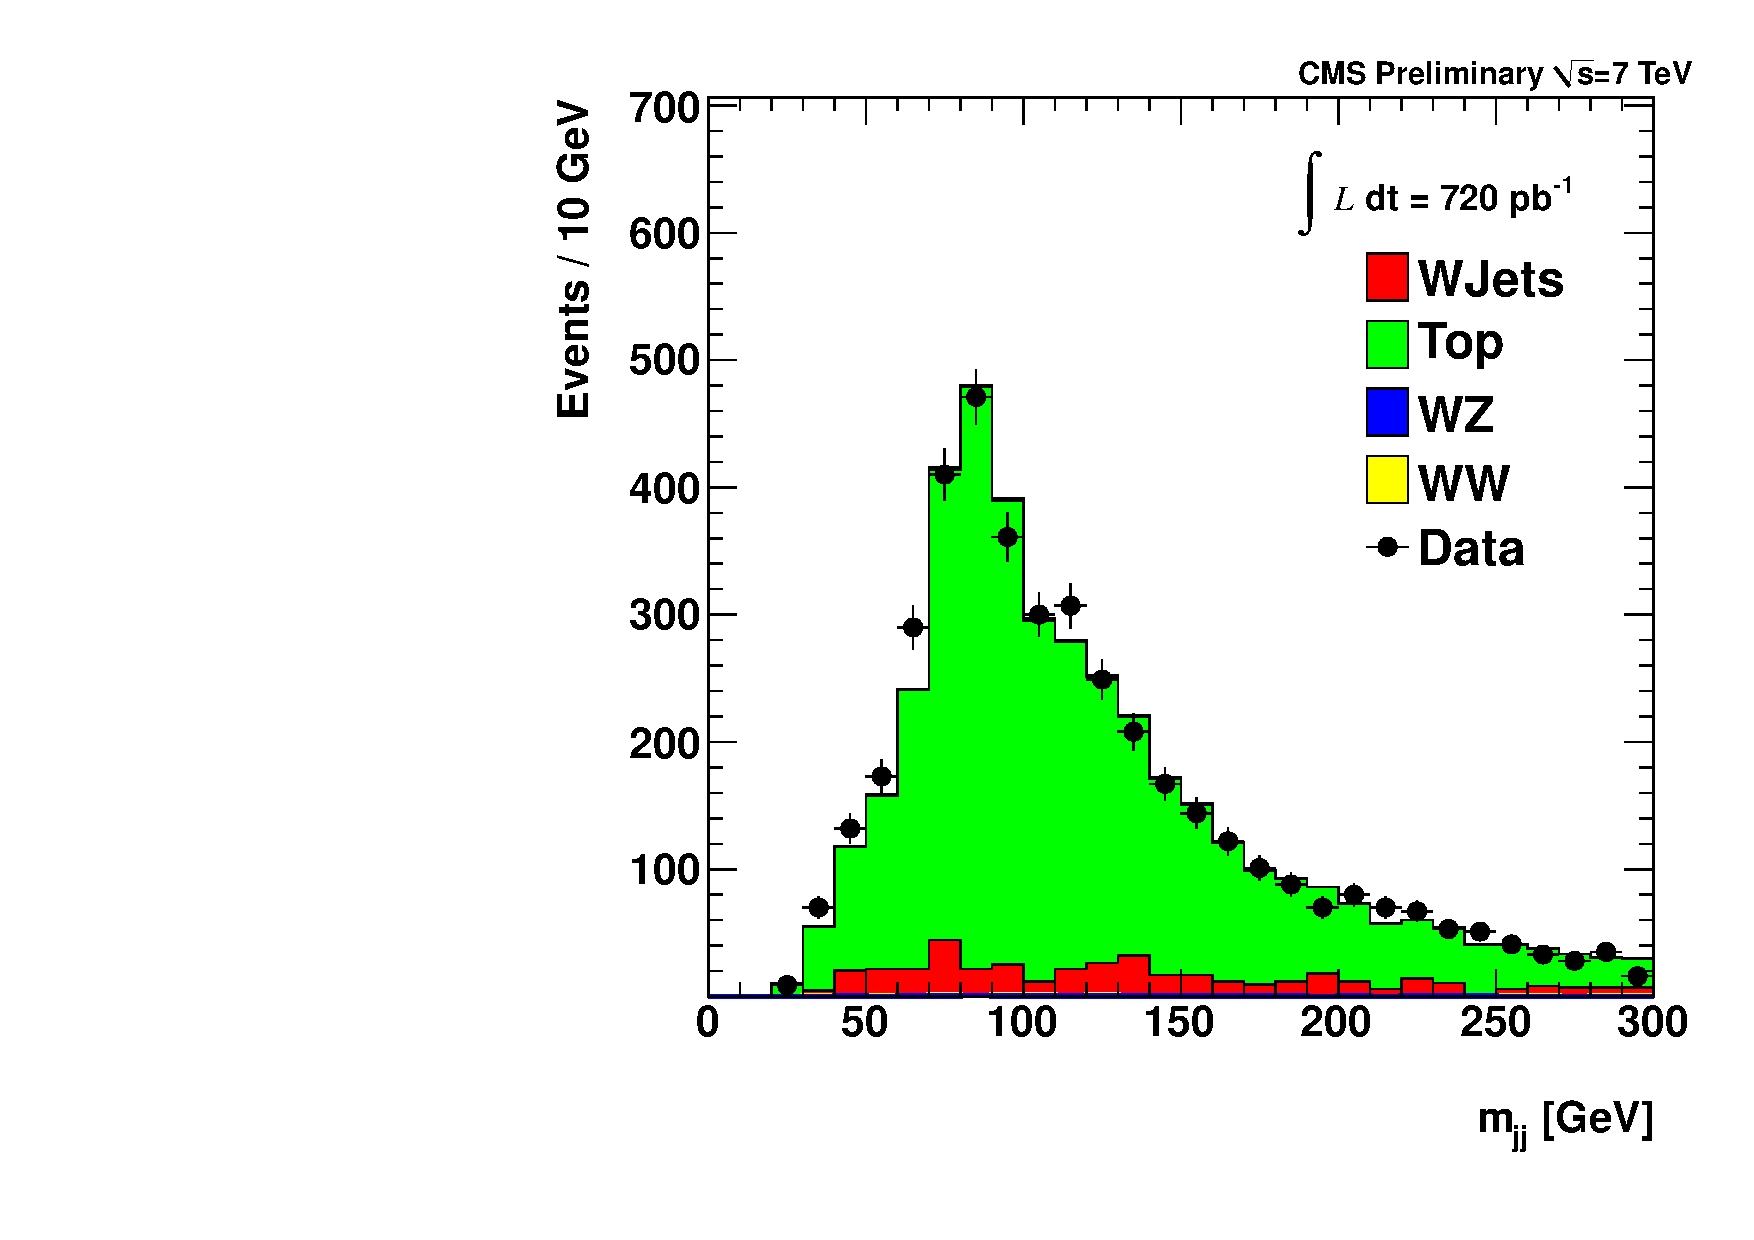
\includegraphics[width=0.48\textwidth]{figures/mJJ-mu-top.pdf}
\put(-0.80,0.0){(a)} 
\unitlength=0.33\linewidth
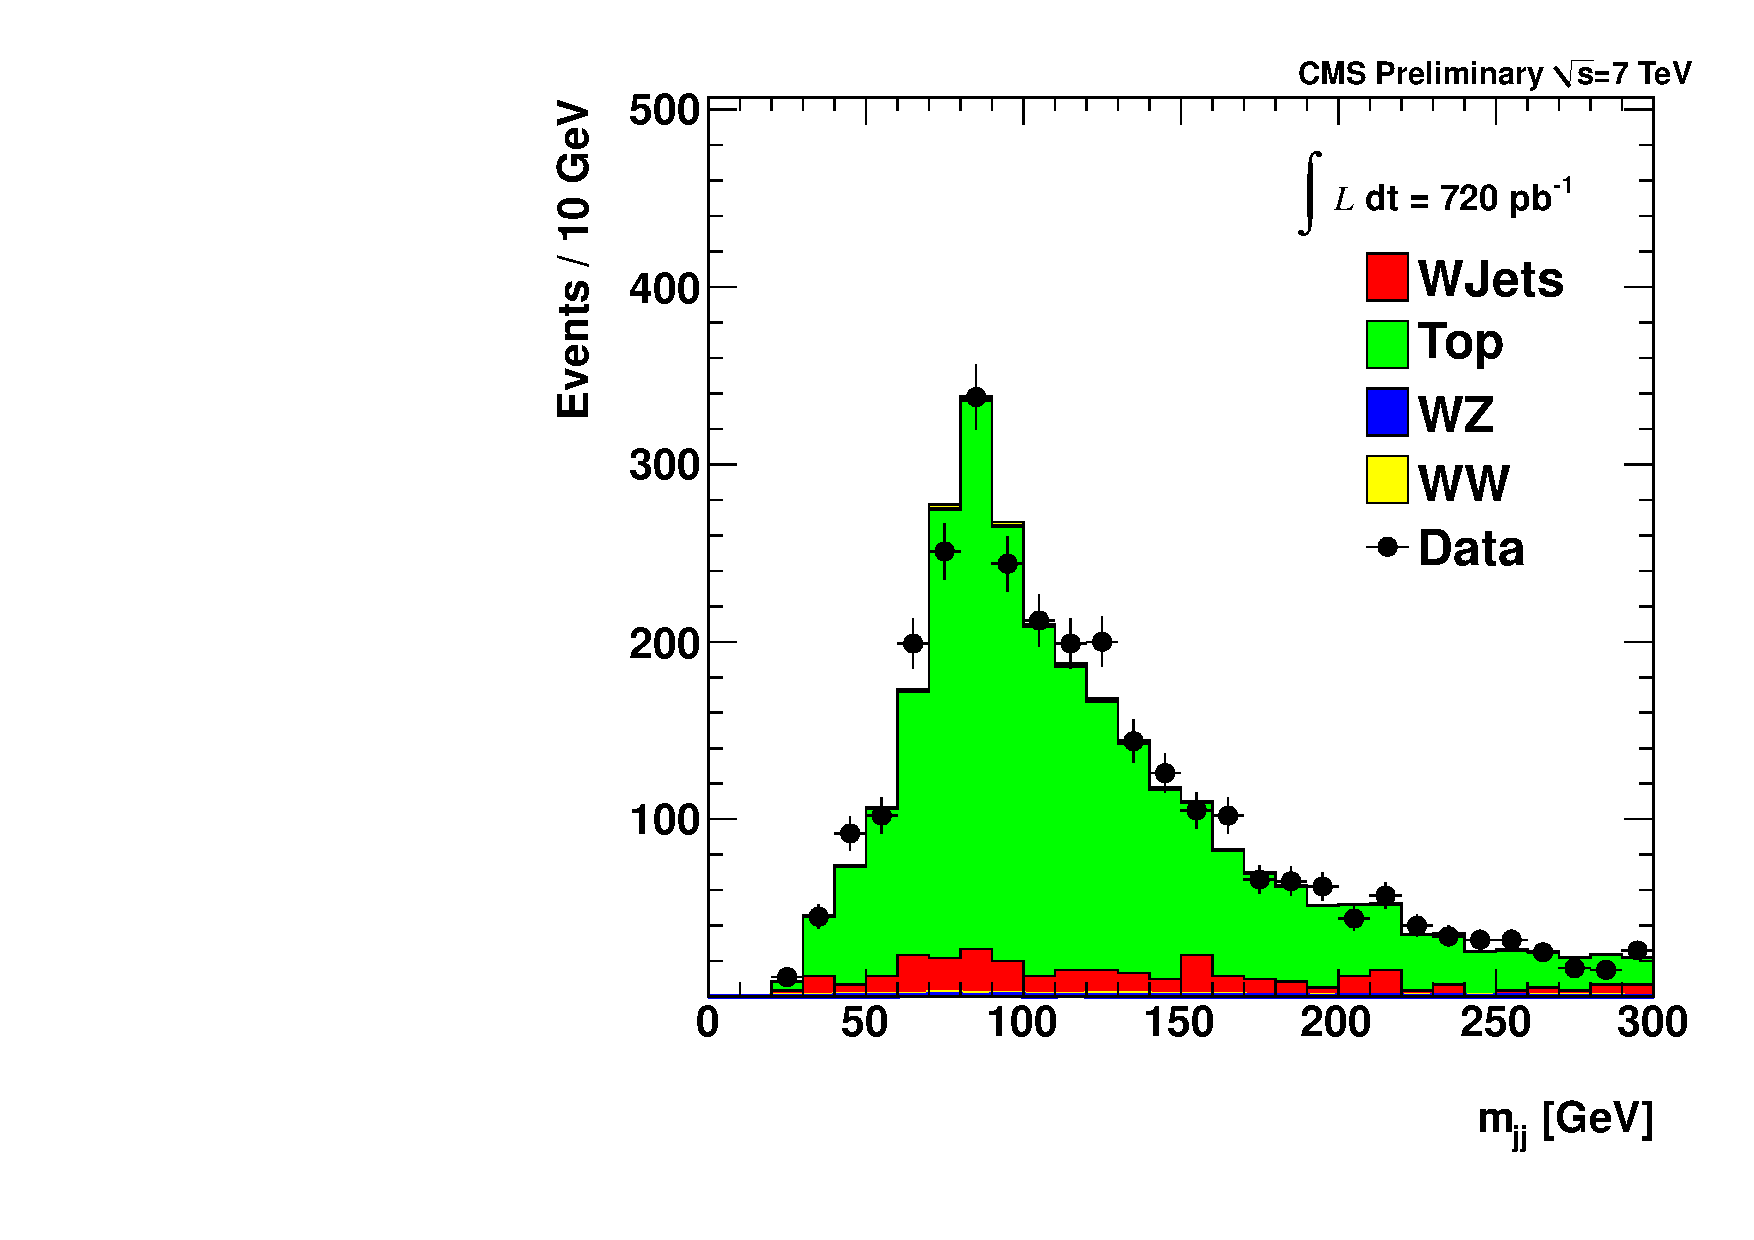
\includegraphics[width=0.48\textwidth]{figures/mJJ-ele-top.pdf}
\put(-0.80,0.0){(b)} 
\caption{
The invariant mass distribution of the two non-$b$-tagged jets in 
events containing a high energy lepton, large $\met$, 
and four jets of which two are $b$-tagged. This sample is dominated 
by $\ttbar$ events. The distribution shown here for both lepton channels 
(a: muon, b: electron) essentially 
establishes how well we can reconstruct a hadronically decaying 
vector boson in CMS detector. The resolution of the reconstructed 
vector boson is dominated by the jet energy resolution.} 
\label{fig:mjj_top}}
\end{figure}
%%%%%%%
%%%%%%%%%%%%%%%%%%%%%%%%%%%%%%%%%%%%%%%%%%%%%%%%%%%%%%%%
\subsection{Dijet mass distribution\label{sec:mjj}}
The dijet invariant mass distribution after all selection criteria 
is shown in Figure~\ref{fig:mjj_DataMCStacked} for muon and 
electron data samples separately. 
The expectation from Monte Carlo is overlaid after adjusting 
the MC for overall difference in reconstruction efficiency 
between data and MC.
The distribution in both muon and electron data 
is consistent with MC expectation for $WW$ and $WZ$ production.
%%%%%%%%%%%%%%%%%%%%%%%%%%%%
%%%%%%%%%%%%%%%%%%%%%%%%%%%%
\begin{figure}[h!] {\centering
\unitlength=0.33\linewidth
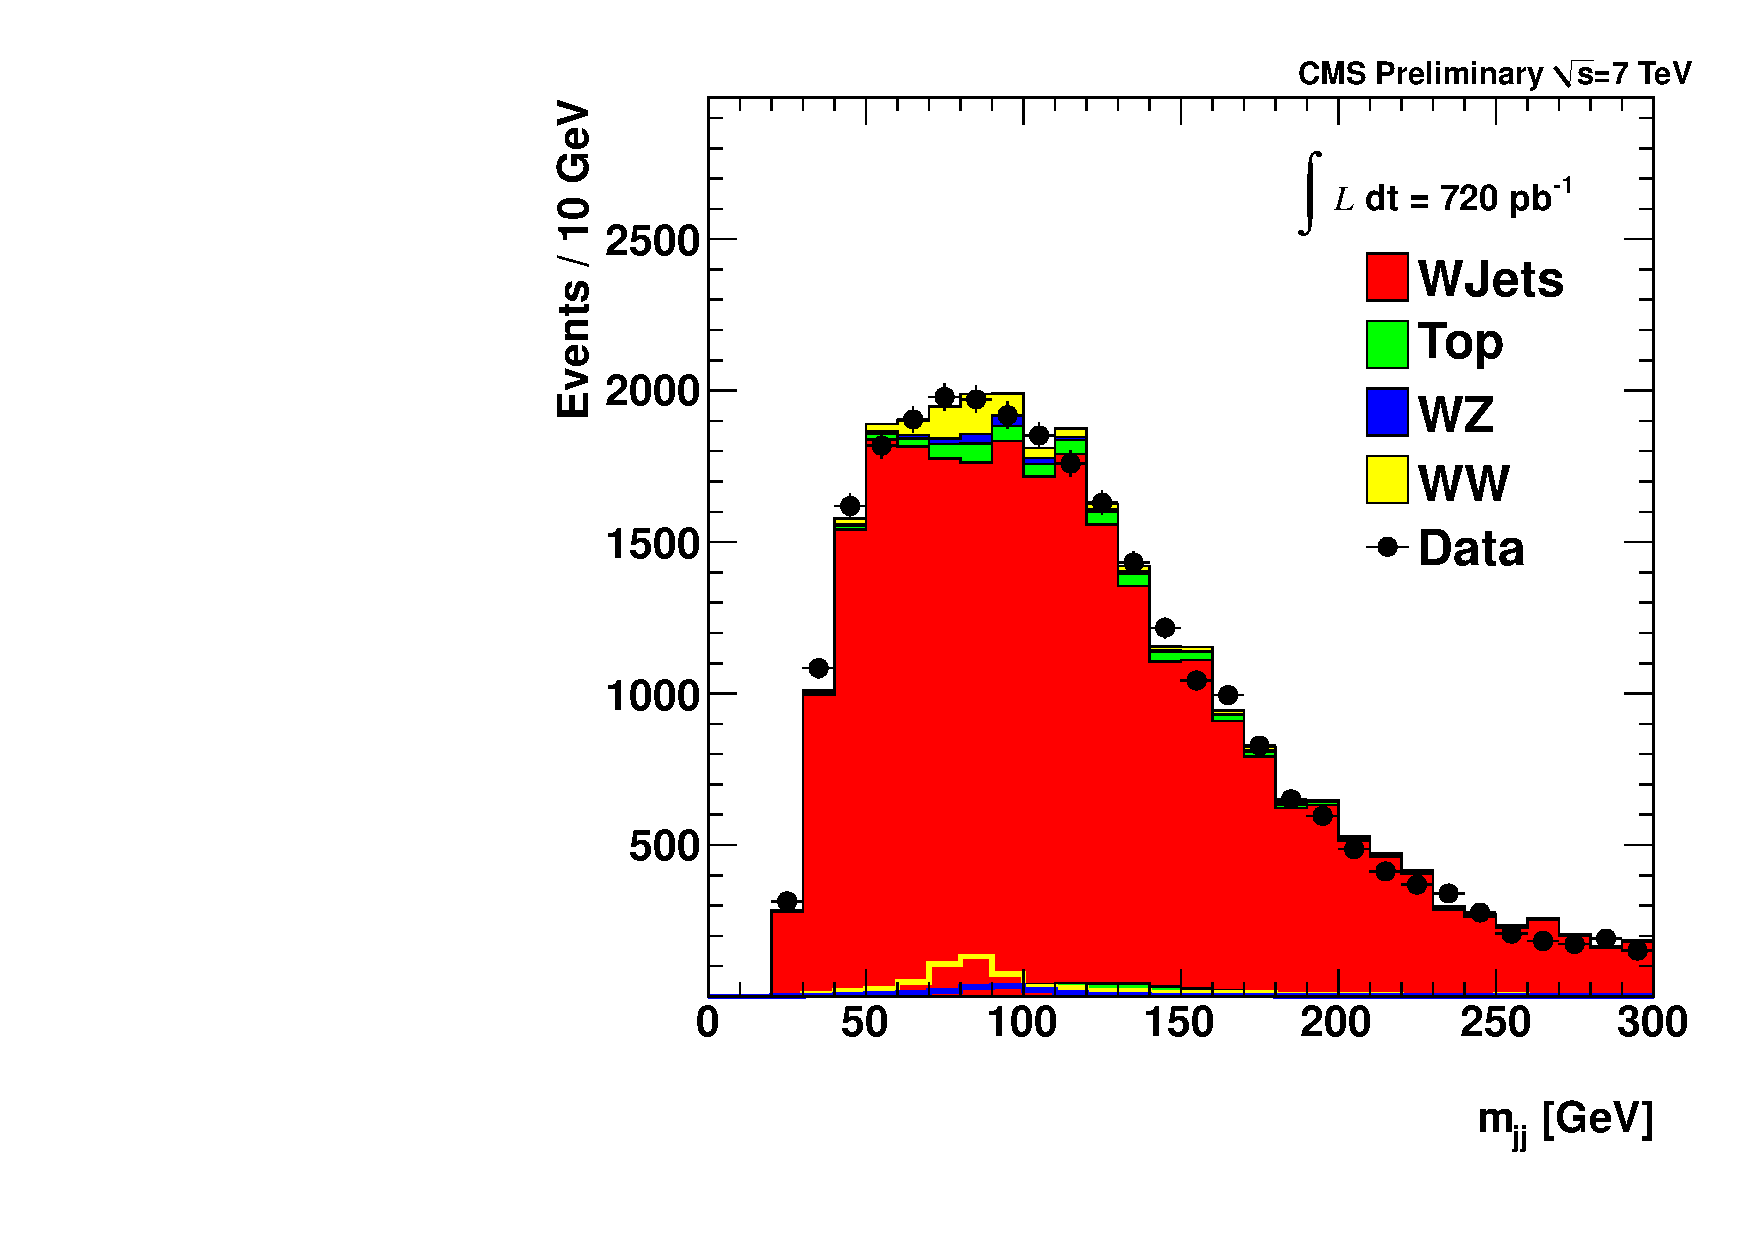
\includegraphics[width=0.48\textwidth]{figures/mJJ-mu-DataMCStacked.pdf}
\put(-0.80,0.0){(a)} 
\unitlength=0.33\linewidth
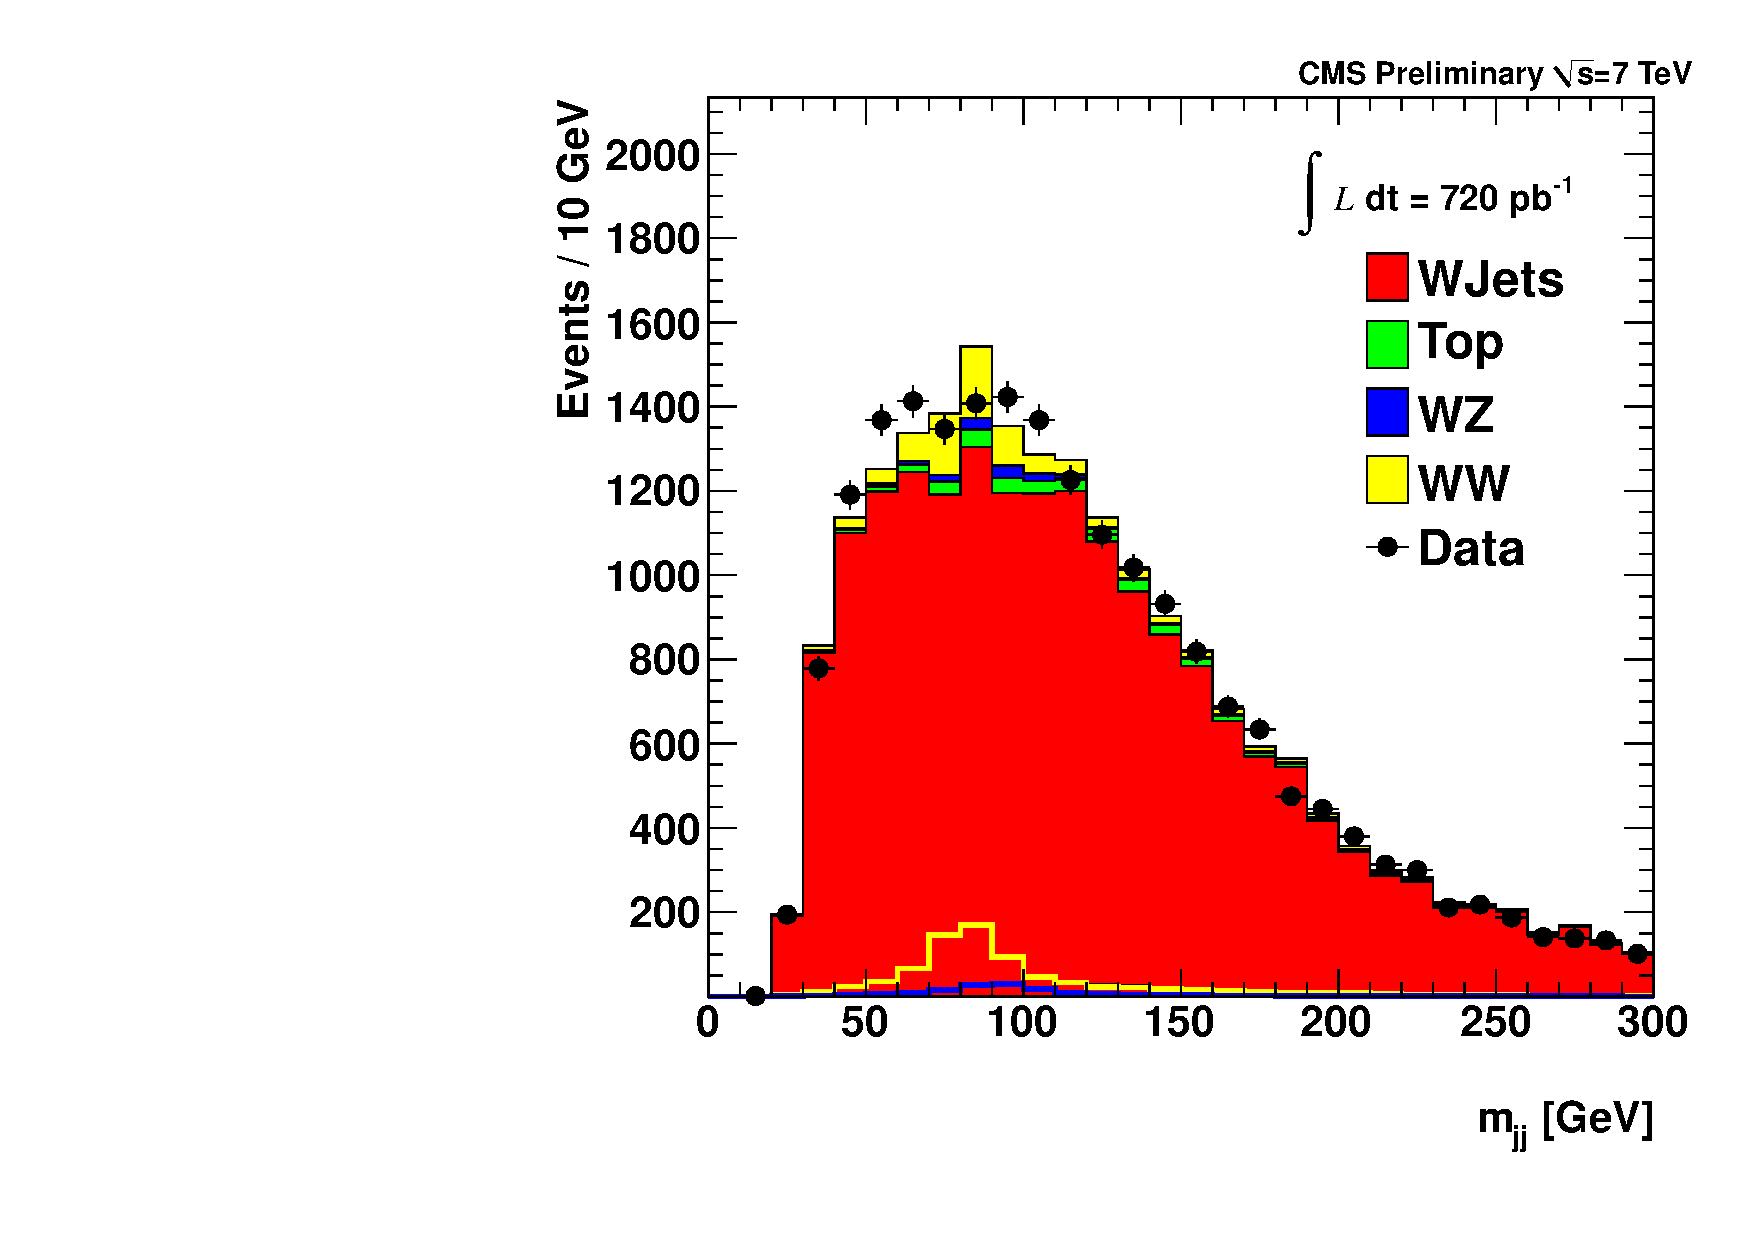
\includegraphics[width=0.48\textwidth]{figures/mJJ-ele-DataMCStacked.pdf}
\put(-0.80,0.0){(b)} 
\caption{
The dijet invariant mass distribution after analysis level selection in 
(a) muon and (b) electron data samples. The expectation from Monte 
Carlo is overlaid. The MC has beed adjusted for overall difference 
in reconstruction efficiency between data and MC.
The uncertainty on data points is statistical only.
} 
\label{fig:mjj_DataMCStacked}}
\end{figure}
%%%%%%%%%%%%%%%%%%%%%%%%%%%%
%%%%%%%%%%%%%%%%%%%%%%%%%%%%%%%%%%%%%%%%%%%%%%%%%%%%%%%%
\subsection{Diboson signal extraction\label{sec:sigExtr}}
We perform a likelihood fit of the $m_jj$ distribution for the electron 
and muon samples combined (and also separately for each as cross check).
The fit is performed in the $m_jj$ region [30,250] GeV and estimates the 
fractions of diboson, $W$+jets, QCD, and top backgrounds using $m_jj$ 
templates obtained from the CMS full simulation. 
The total diboson and $W$+jets contribution are free parameters of the fit 
while top and single top ontribution are constrained to the measured 
cross section. 
The QCD multi-jet background is insignificant, however, we plan to 
constrain its contribution by performing a fit to the the $\met$ distribution. 


The dijet invariant mass distribution for the sum of electron 
and muon events after fit is shown in Figure~\ref{fig:CombinedFit}. 
The diboson peak is prominently visible here.
We plot the $m_jj$ distribution in data after subtracting all 
background components.
Figure~\ref{fig:CombinedFitSubtracted} shows the distribution 
after subtraction of fitted background components obtained in 
Figure~\ref{fig:CombinedFit}.
%%%%%%%%%%%%%%%%%%%%%%%%%%%%
%%%%%%%%%%%%%%%%%%%%%%%%%%%%
%%%%%%%
\begin{figure}[h!] {\centering
\unitlength=0.33\linewidth
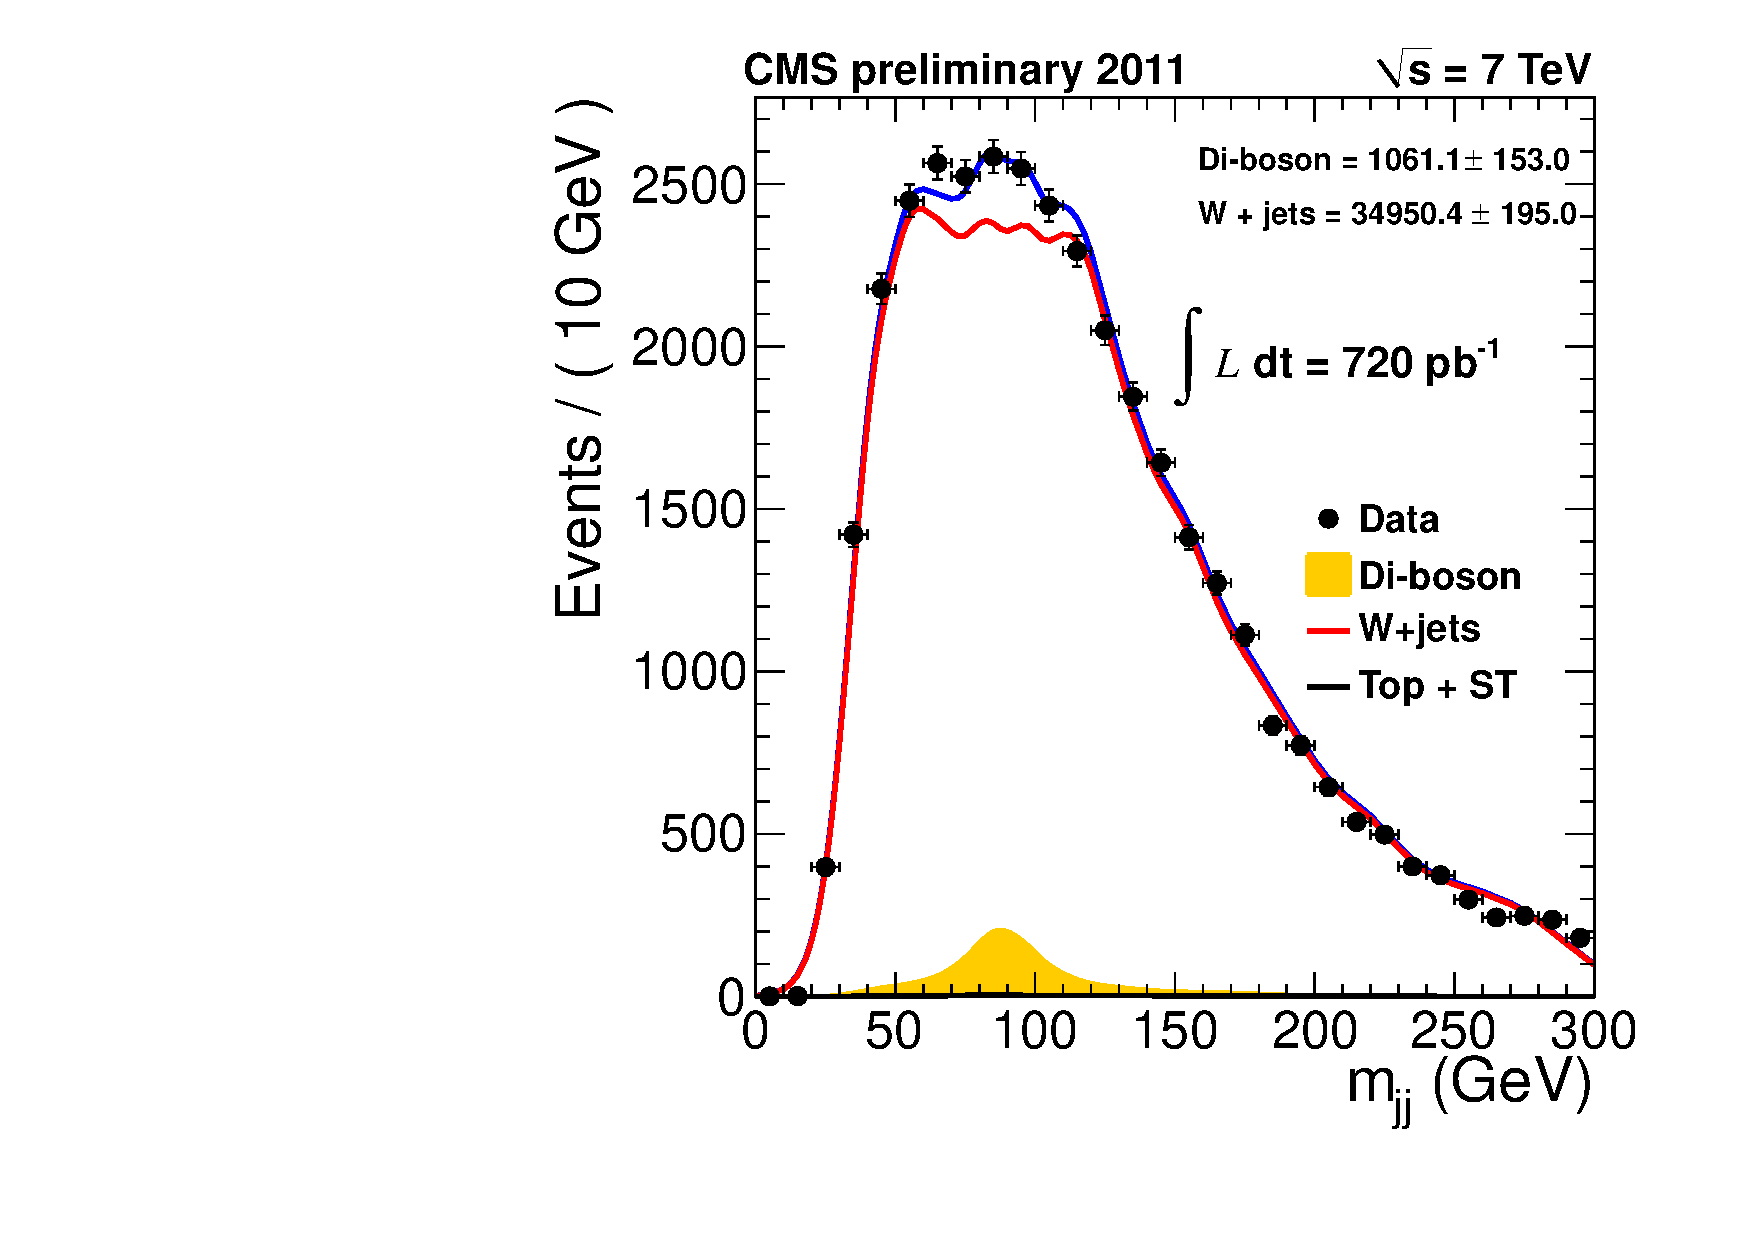
\includegraphics[width=0.48\textwidth]{figures/mJJ-combined-fit.pdf}
\put(-0.80,0.0){(a)} 
\unitlength=0.33\linewidth
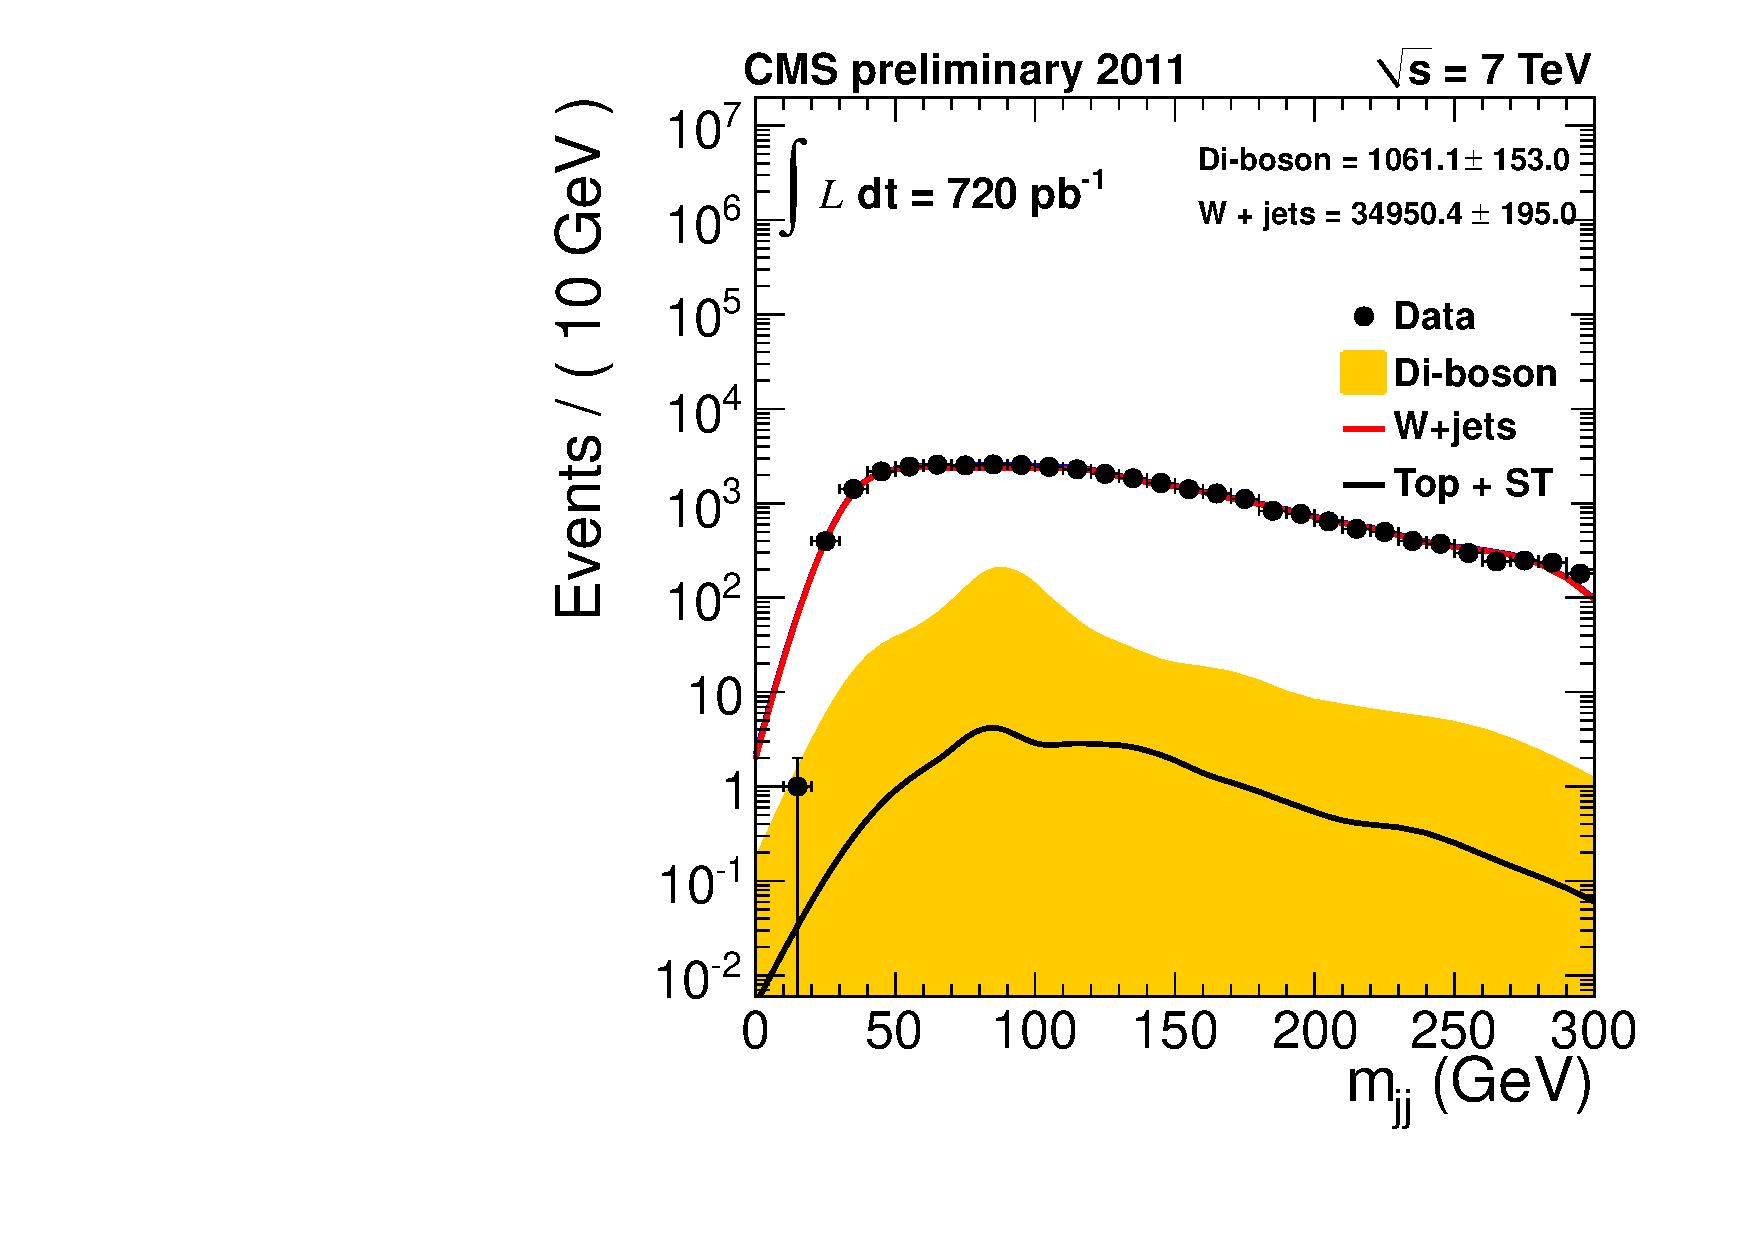
\includegraphics[width=0.48\textwidth]{figures/mJJ-combined-fit-logY.pdf}
\put(-0.80,0.0){(b)} 
\caption{
Projection of the $m_jj$ fit  to extract diboson signal for the sum 
of electron and muon events  (a) on linear scale and 
(b) on logarithmic scale.} 
\label{fig:CombinedFit}}
\end{figure}
%%%%%%%
%%%%%%%
\begin{figure}[h!] {\centering
    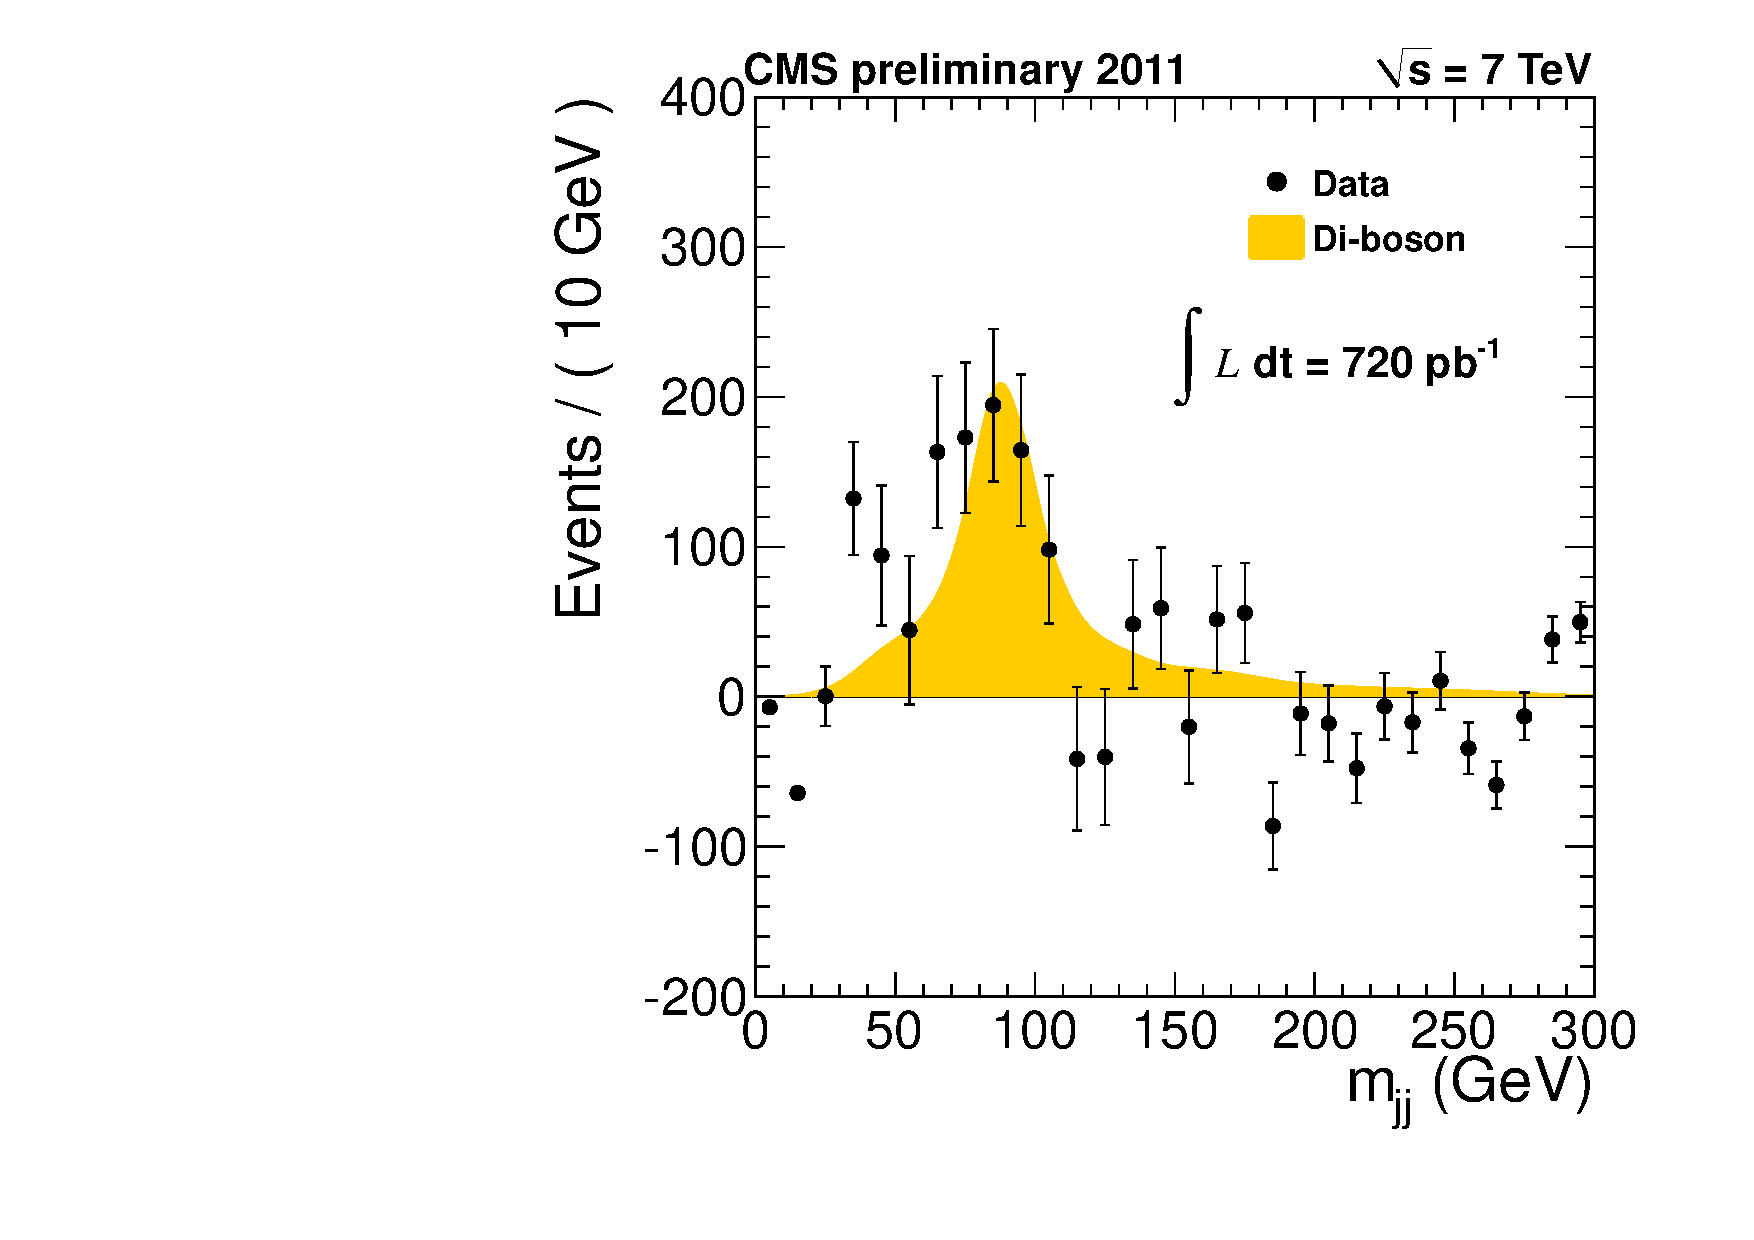
\includegraphics[width=0.5\textwidth]{figures/mJJ-combined-fit-subtracted.pdf}
    \caption{The dijet invariant mass distribution for the sum of 
      electron and muon events after subtraction of fitted 
      background components obtained in Figure~\ref{fig:CombinedFit}.}
    \label{fig:CombinedFitSubtracted}}
\end{figure}
%%%%%%%
%%%%%%%%%%%%%%%%%%%%%%%%%%%%%%%%%%%%%%%%%%%%%%%%%%%%%%%%
\subsection{Systematic uncertainties\label{sec:syst}}
We consider several sources of systematic uncertainty, taking into account 
their effect on both the signal acceptance and on template shapes for the 
signal extraction fit. 
The uncertainty on the normalization of the backgrounds is taken as part of 
the statistical uncertainty. 
The largest sources of systematics are due to the shape uncertainty of the 
$W$+jets template. 
Other sources of systematics considered are the jet energy scale (JES) and 
resolution (JER), initial and final state radiation (ISR and FSR), PDFs, 
jet energy resolution and trigger and lepton identification efficiency. 
Finally, another important contribution to the cross section 
systematics is due to luminosity measurement uncertainty. 

\par
We perform a number of pseudo experiments to verify that 
the signal extraction procedure is unbiased and statistical 
uncertainties reported have good coverage.


\par
By far the largest uncertainty in diboson signal extraction comes 
from the imperfect understanding of the $W$+jets background shape.
We plan to try $W$+jets template from several different Monte Carlo 
generators (\textit{e.g.,} \textit{MadGraph}, \textit{Sherpa}, 
\textit{MCFM}) to assess the overall systematics from the 
imperfect understanding of the $W$+jets spectrum and due to NLO 
effects.
We also plan to cross check by using data-driven techniques 
(\textit{e.g.}, by constraining the template in the sidebands 
or by using $m_{jj}$ template from $Z$+jets events which have 
similar kinematics).

%--------------------------------------------------
\par
Small difference in lepton energy scale and resolution and 
also in lepton selection and triggering efficiency between data and 
Monte Carlo simulation is a source of systematic uncertainty. 
This arises because we take the signal and background shapes 
from simulation and use these to fit the data for extracting signal 
yield. 
We perform several iterations of the likelihood fit using modified 
shapes that account for these differences, and take the largest 
variation in signal yield as systematic uncertainty.


%--------------------------------------------------
\par
The systematic uncertainty due to jet energy scale and jet 
resolution affects the signal acceptance and $m_{jj}$ distribution.
The main uncertainty in jet reconstruction comes from jet 
energy scale uncertainty, while the uncertainty on the 
resolution contributes a much smaller effect.
Preliminary estimate with 2010 data show that jet energy 
uncertainty could be kept within about 4\% and resolution within 10\%.
For more details see Refs.~\cite{jme-10-010,jetsyst2}.


We account for this systematics by including jet energy scale 
and resolution uncertainties as parameters in the likelihood. 
We let these parameters vary in the fit within the allowed 
uncertainty range quoted above. 
The fit finds the best values for these parameters allowed by 
our data, and their uncertainty gets propagated into the 
statistical uncertainty of the signal yield reported by the fit.


Our preliminary estimates show that JES
variation by $\pm 1\sigma$ changes the acceptance for the  
diboson events by about xxx\%.

%--------------------------------------------------
\par
Uncertainty in the $\met$ measurement also affects directly our 
signal acceptance. 
Again we vary the uncertainty by $\pm 1\sigma$  and compute the change 
in acceptance.

%--------------------------------------------------
\par
Uncertainty in the the cross sections of insignificant backgrounds 
like $\ttbar$ and single top need to be propagated to the 
final result.
Finally, we propagate the uncertainty in the LHC luminosity -- the latest 
estimation being 6$\%$ -- as a systematic uncertainty in the measurement.
%%%%%%%%%%%%%%%%%%%%%%%%%%%%%%%%%%%%%%%%%%%%%%
%%%%%%%%%%%%%%%%%%%%%%%%%%%%%%%%%%%%%%%%%%%%%%
\subsection{Result and conclusions\label{sec:conclusion}}
In summary, we have presented the first study of the standard model 
electroweak production of the $WW/WZ\to\ell\nu jj$ processes in CMS. 
The data used in this analysis are from LHC runs 2010 and 2011 (until the 
end of June, 2011), and correspond to an 
integrated luminosity of 1 fb${}^{-1}$. 
We consider a data sample of high-$p_T$ electrons and muons to reconstruct 
the leptonically decaying $W$ boson. 
We look for another boson candidate in the event by selecting two 
additional jets. 
In order to extract our diboson signal, a fit to the invariant mass 
distribution $m_{jj}$ of the two jets is performed. 

\par
We have established the observation of diboson signal in non purely-leptonic 
final states. We find $xxx \pm yyy$ $WW/WZ\to\ell\nu jj$ events. 
We measure the production cross-section to be 
$\sigma(WW/WZ)$ = $xxx \pm yyy$(stat.) $\pm zzz$(syst.). 
These results are preliminary.
The results are consistent with the expectations of the standard model 
at next-to-leading order in perturbative QCD calculations.


